\clearpage
\section{Результати}
\label{sec:results}

\subsection{Одиничний експорт із кліки}
\label{sec:res_clique}

\emph{Часи експорту з джерела, яке швидко насичується, добре узгоджуються, але агрегований інтерфейс допускає неможливі порядки передачі.} У тесті «кліка--листок» (рисунок~\ref{fig:clique_leaf}) середні часи експорту становили 110.18 (\Full{}) і 112.62 (\TS{}); парна різниця $+2.43$ мала бутстреп-інтервал $[-0.35,5.27]$. Емпіричні функції розподілу майже збігаються ($W_1=3.25$, тобто $\eW=2.95\%$; відстань Колмогорова--Смирнова 0.0142, асимптотичне $p\approx0.27$). Із середнього часу експорту близько 110 лише $\mathbb{E}[T_B]=8.36$ у середньому потрібно, щоб заразити перший вузол-мост~\eqref{eq:clique_TB}; решта припадає на очікування передачі через інтерфейс з інтенсивністю не більшою за $k\beta=0.01$. Отже, період, протягом якого стани межі й усієї спільноти відрізняються, короткий, а агрегований годинник близький до точного, як випливає з твердження~\ref{prop:ordering} та~\eqref{eq:hazard_variance}.

Водночас діагностика порядку розрізняє моделі: у 98 із 10\,000 запусків \TS{} (0.98\%) листок було заражено раніше за обидва вузли-мости, чого ніколи не трапляється у \Full{} (рисунок~\ref{fig:clique_leaf}b,c). На середній панелі показано $T_{\mathrm{export}}-T_B$: фізичний час очікування у \Full{}, але знаковий діагностичний показник порядку у \TS{}.

\clearpage
\begin{figure}[H]
\centering
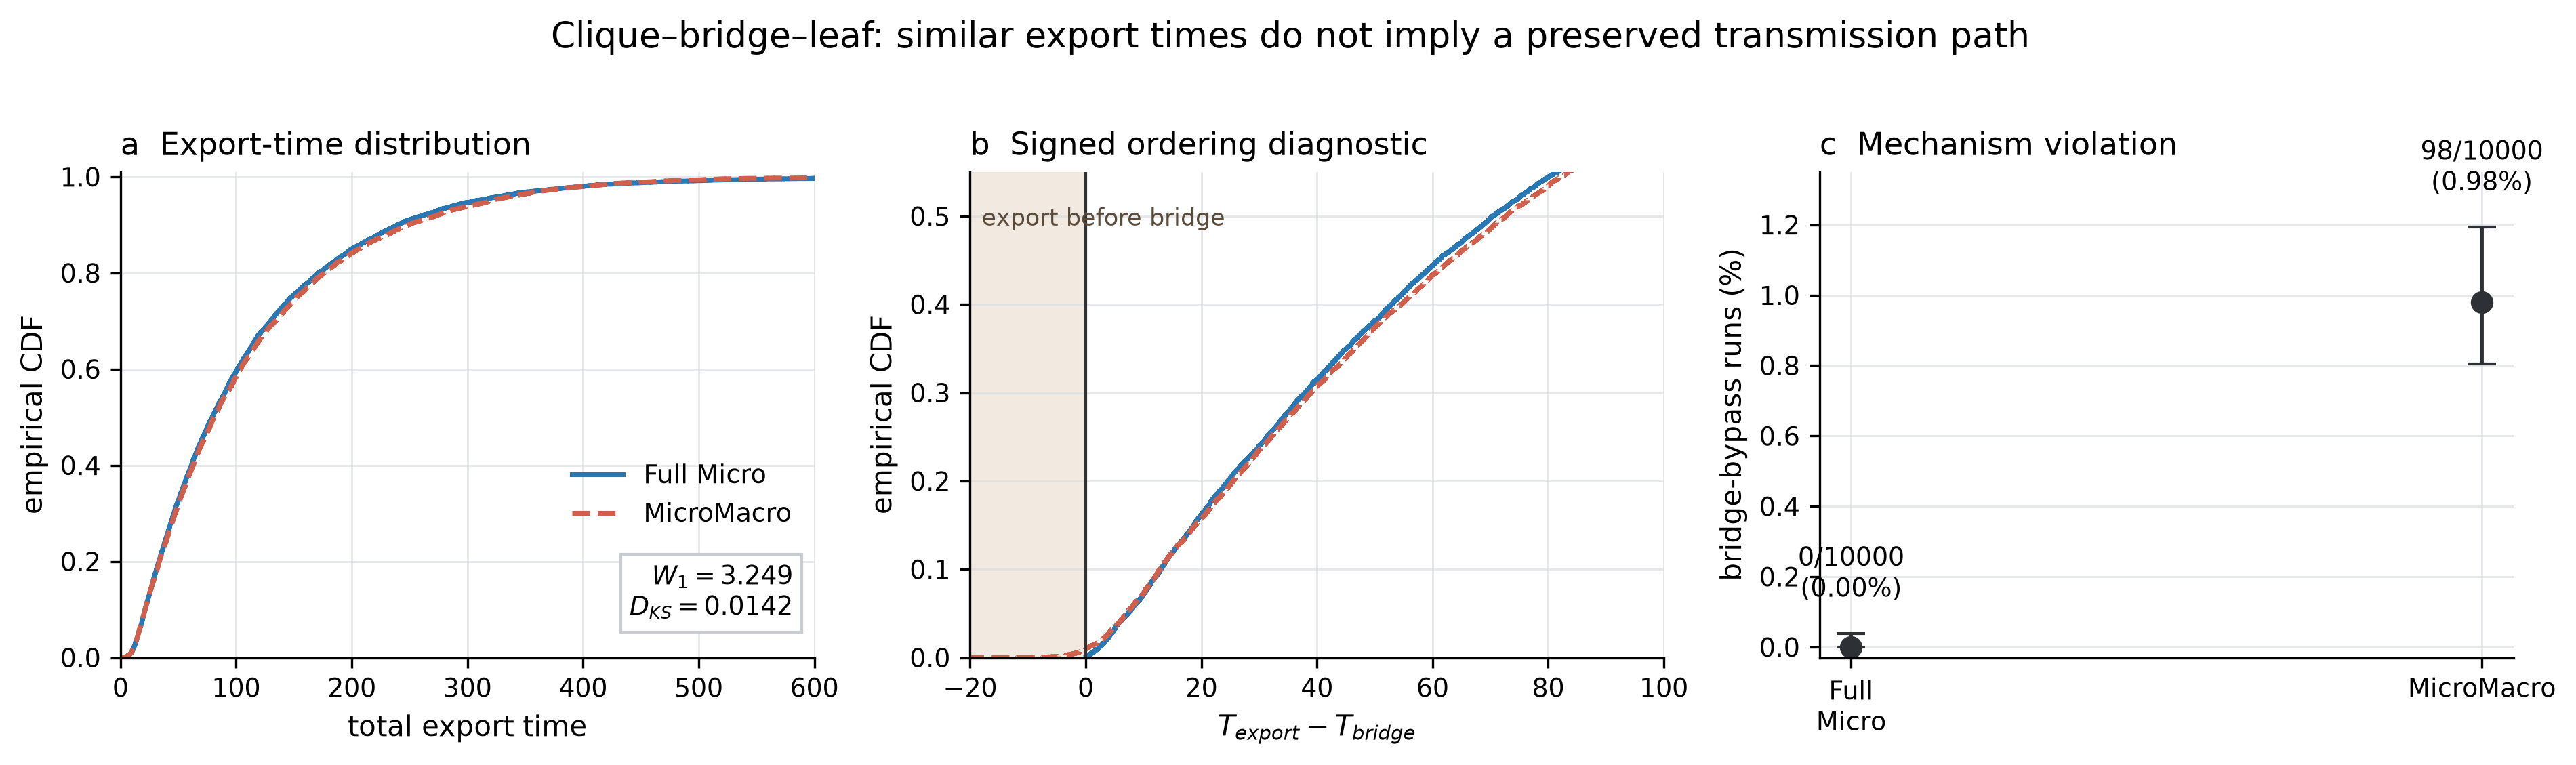
\includegraphics[width=\linewidth]{Images/clique_leaf/clique_leaf_endpoint_and_mechanism.png}
\caption{Тест «кліка--листок» ($n=100$, $k=2$, $\beta=0.005$, 10\,000 запусків для кожної моделі). (a) Емпіричні функції розподілу часу експорту. (b) Емпіричні функції розподілу $T_{\mathrm{export}}-T_B$; від'ємні значення (заштрихована область) відповідають експорту до зараження будь-якого вузла-моста. (c) Частка таких запусків з обходом мостів із 95\% інтервалами. ``Full Micro'' позначає \Full{}, а ``MicroMacro'' --- \TS{}.}
\label{fig:clique_leaf}
\end{figure}

\subsection{Одиничний експорт зі зв'язних випадкових джерел}
\label{sec:res_source}

\emph{Зі збільшенням довжини внутрішніх шляхів обхід мостів стає поширеним, а агрегований експорт відбувається раніше, як передбачає твердження~\ref{prop:ordering}.} На рисунку~\ref{fig:source_sweep} показано серію експериментів «джерело--листок». Середні часи активації мостів у двох моделях були подібними: різниця не перевищувала 7\% для кожного ASPL (наприклад, 1165 і 1136 за ASPL 6, $k=1$), як і очікувалося через однакову локальну динаміку до експорту. У \Full{} за $k=1$ очікування після активації моста залишалося в межах 322--359 за кожного ASPL, що узгоджується з $\mathrm{Exp}(\beta)$ із середнім 333. У \TS{} знаковий інтервал $T_{\mathrm{export}}-T_B$ ($k=1$) зменшився приблизно з 340 у щільних джерелах до 207--295 за ASPL $\ge5$, оскільки агрегована інтенсивність накопичувалася ще до того, як справжній міст ставав інфекційним.

\clearpage
\begin{figure}[H]
\centering
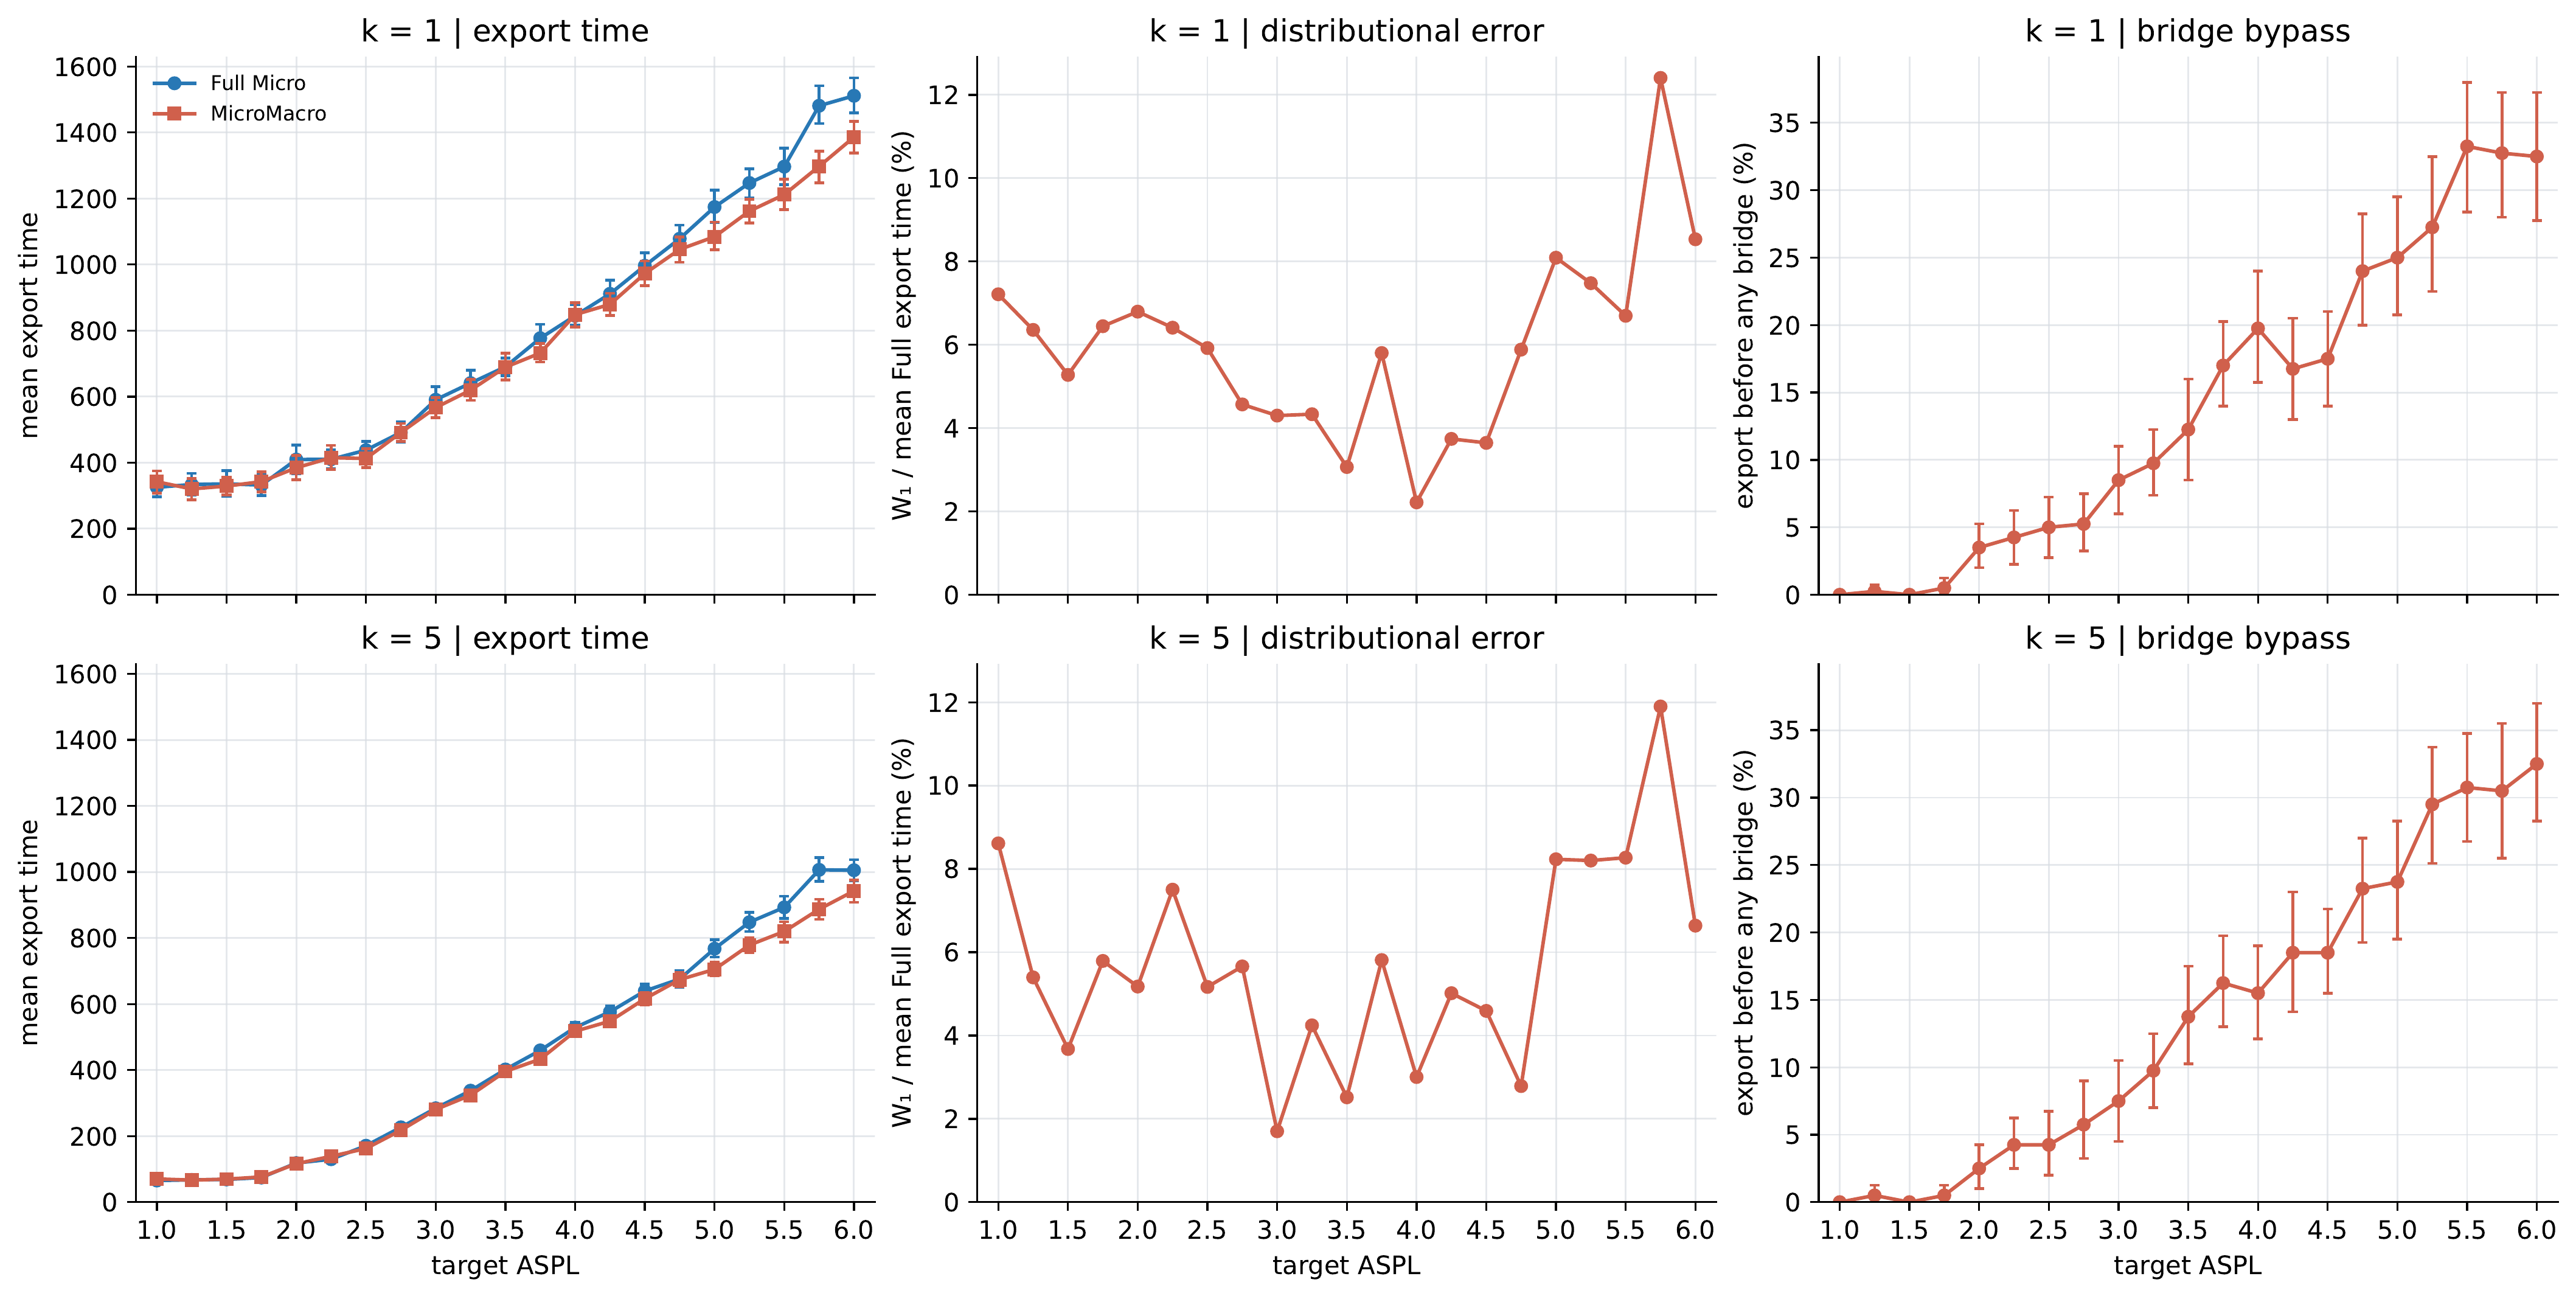
\includegraphics[width=\linewidth]{Images/fig_aspl_export_fidelity.png}
\caption{Серія експериментів «джерело--листок»: $n=1000$, $\beta=0.003$, $k=1$ (угорі) та $k=5$ (унизу), 400 парних запусків для кожної точки. Ліворуч: середній час експорту. У центрі: відносна відстань Васерштайна $\eW$ між розподілами часу експорту. Праворуч: частка експортів \TS{}, що передували зараженню першого моста; у \Full{} таких випадків не було. Відрізки похибок --- 95\% інтервали блокового бутстрепу. ``Full Micro'' позначає \Full{}, а ``Production MicroMacro'' --- \TS{}.}
\label{fig:source_sweep}
\end{figure}

Частка обходів зросла від не більш як 0.5\% за ASPL $\le1.75$ до 19.75\% (95\% інтервал 15.8--24.0\%) за ASPL 4 і $k=1$, а за ASPL 6 --- до 32.5\% для обох ширин інтерфейсу. Зсув середнього часу експорту був статистично відмінним від нуля, з інтервалами, що не містили нуль, для обох ширин за кожного ASPL $\ge5$. Його значення були в межах від $-6.2\%$ до $-12.4\%$; за ASPL 6 вони становили $-8.3\%$ ($[-13.1,-3.5]$) для $k=1$ і $-6.2\%$ ($[-10.3,-2.3]$) для $k=5$. Нижче ASPL 5 статистично відмінний від нуля зсув виявлено лише для $k=5$ за ASPL 3.75, 4.25 і 4.5 (від $-3.7\%$ до $-5.8\%$). У жодній точці серії не виявлено додатного зсуву, що узгоджується з напрямом, передбаченим твердженням~\ref{prop:ordering}.

Нерегулярну центральну панель слід тлумачити обережно. Для майже експоненційних часів експорту та $R=400$ запусків для кожної моделі очікуване $\eW$ двох вибірок з одного розподілу становить приблизно $\sqrt{\pi/R}\approx9\%$ (додаток~\ref{app:floor}). Отже, значення 3.7--8.6\%, спостережені за ASPL $\le1.75$, узгоджуються із суто вибірковою мінливістю. Тому відстані для одиничного експорту слід розглядати разом зі зсувом середнього та його інтервалом. Натомість обхід у \Full{} за побудовою дорівнює нулю, тому кожен спостережений обхід є справжньою розбіжністю. За ASPL 4 він стосується однієї п'ятої експортів, хоча розподіли часу експорту залишаються близькими.

\subsection{Повторні переходи через ланцюг клік}
\label{sec:res_cliques}

\emph{Коли внутрішнє поширення швидке, близьке узгодження зберігається після дев'яти послідовних агрегованих переходів.} У ланцюзі з десяти клік по 1000 вузлів із $k=1$ медіанний час прибуття до останньої спільноти становив 2785 у \Full{} і 2877 у \TS{}, а $\eW=3.34\%$ (рисунок~\ref{fig:chain_cliques}). Пермутаційний поріг для цієї комірки становив 5.1\% ($p=0.32$), тому два термінальні розподіли статистично нерозрізнювані. Функції розподілу перетинаються, отже різниця не є сталим запізненням. Кліка з 1000 вузлів у середньому насичується за $2H_{999}/(\beta n)\approx5$ одиниць часу, тоді як середній час переходу через ребро дорівнює 333 ($\rho=0.002$). Тому агрегована інтенсивність відрізняється від точної лише протягом незначної частини кожного переходу.

\clearpage
\begin{figure}[H]
\centering
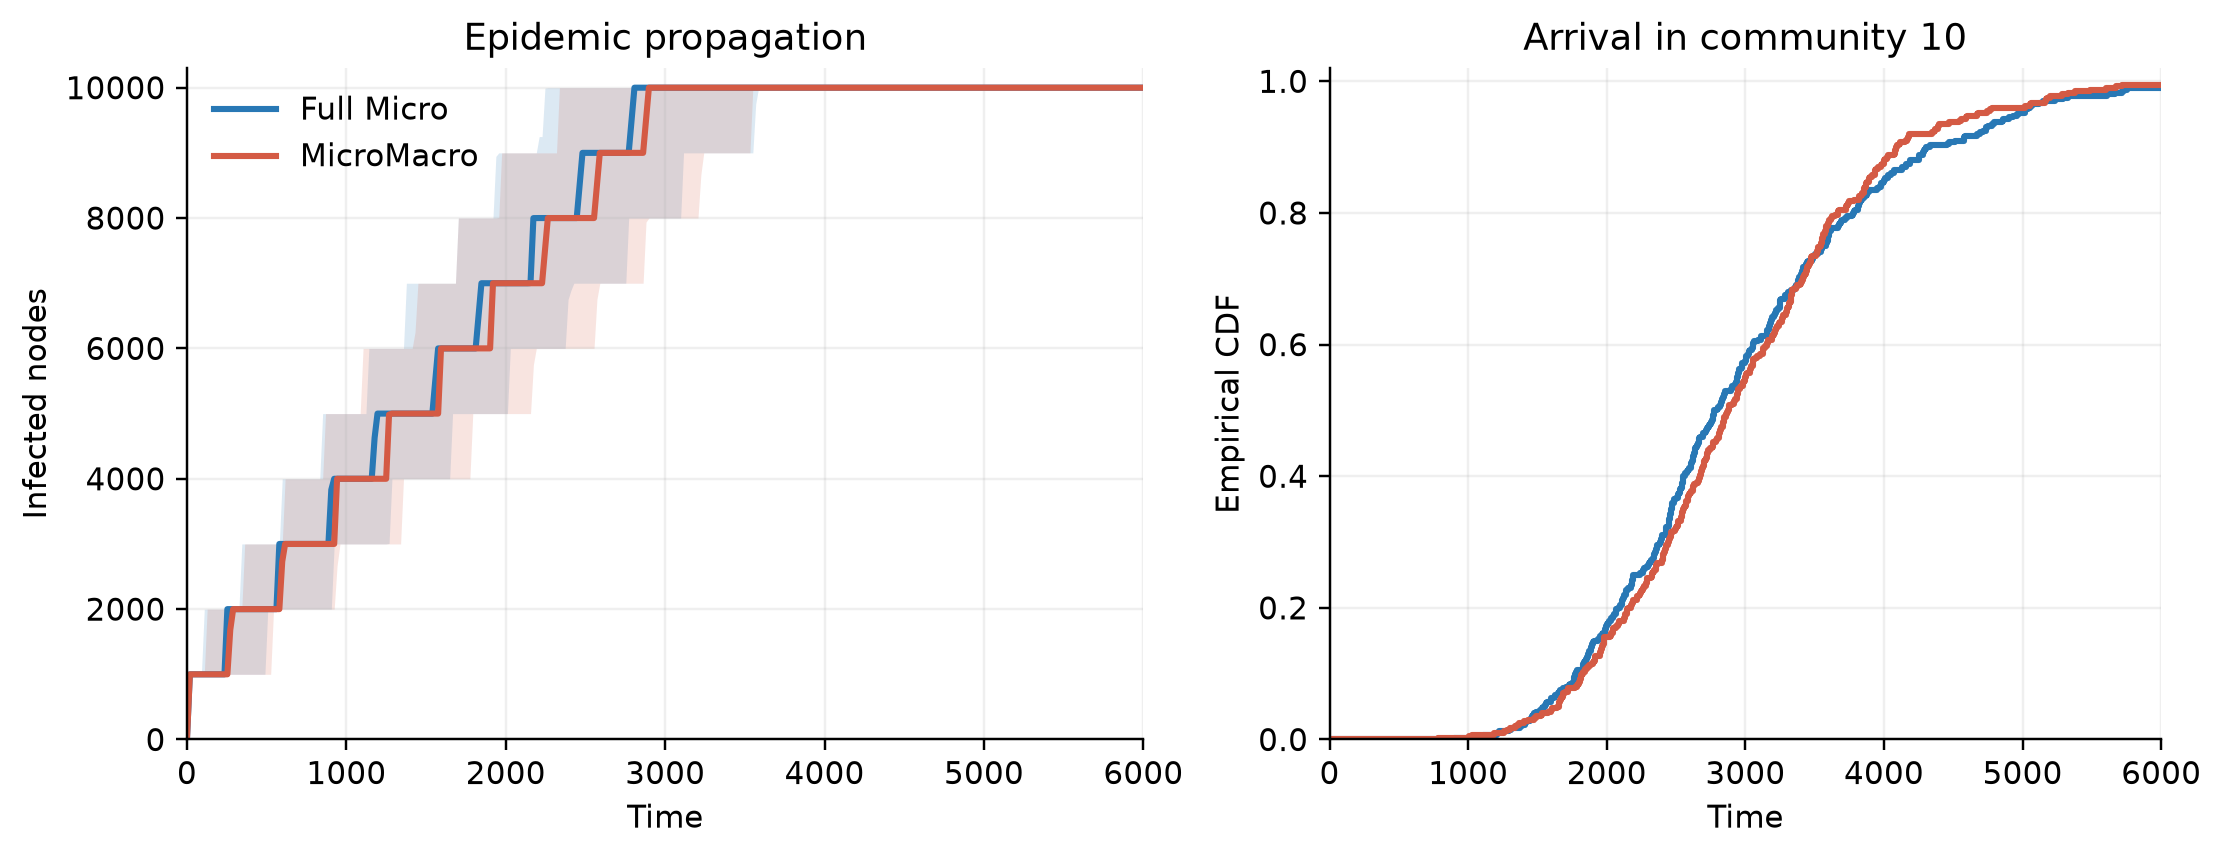
\includegraphics[width=\linewidth]{Images/chain_cliques/chain_cliques_n1000_k1_propagation_cdf_random_initial.png}
\caption{Ланцюг із десяти клік по 1000 вузлів з одним ребром між послідовними кліками ($k=1$, $\beta=0.003$, 400 запусків для кожної моделі). Ліворуч: поточкова медіана кількості інфікованих вузлів із міжквартильними смугами. Праворуч: емпірична функція розподілу часу прибуття до десятої спільноти ($T_9$). Чотири значення прибуття \Full{} і два \TS{} лежать поза показаним діапазоном; усі вони спостережені.}
\label{fig:chain_cliques}
\end{figure}

\subsection{Ланцюги випадкових спільнот}
\label{sec:res_chain_random}

\emph{Розріджені спільноти з довгими шляхами дають систематично ранні прибуття, відносна величина яких залишається сталою вздовж ланцюга, тоді як абсолютне випередження накопичується.} На рисунку~\ref{fig:chain_heatmap} показано кумулятивні часи прибуття у ланцюгах спільнот із 1000 вузлів. Для цільового ASPL 2--3 термінальне $\eW$ становило 1.4--2.5\%, що близько до його вибіркового порога. За ASPL 6 модель \TS{} досягала останньої спільноти раніше на 13.9\% за медіаною для $k=1$ і на 10.7\% для $k=5$ ($\eW=13.6\%$ і 10.9\%). У рядку ASPL 5 за $k=1$ відносне медіанне випередження становило близько 10\% як у першій, так і в останній спільноті, тоді як його абсолютна величина зросла приблизно зі 107 до 1018 одиниць часу. Отже, стала відносна похибка вздовж ланцюга означає зростання абсолютної похибки у віддалених спільнотах. Додатні значення у першому стовпці рядка клік ($+12.6\%$ і $+11.5\%$) не є статистично відмінними від нуля: для $k=1$ зсув середнього першого переходу дорівнює $+4.9\%$ із 95\% інтервалом $[-8.0,18.3]\%$. Для одиничних переходів також характерний вищий вибірковий поріг відстаней, ніж для кумулятивних.

\clearpage
\begin{figure}[H]
\centering
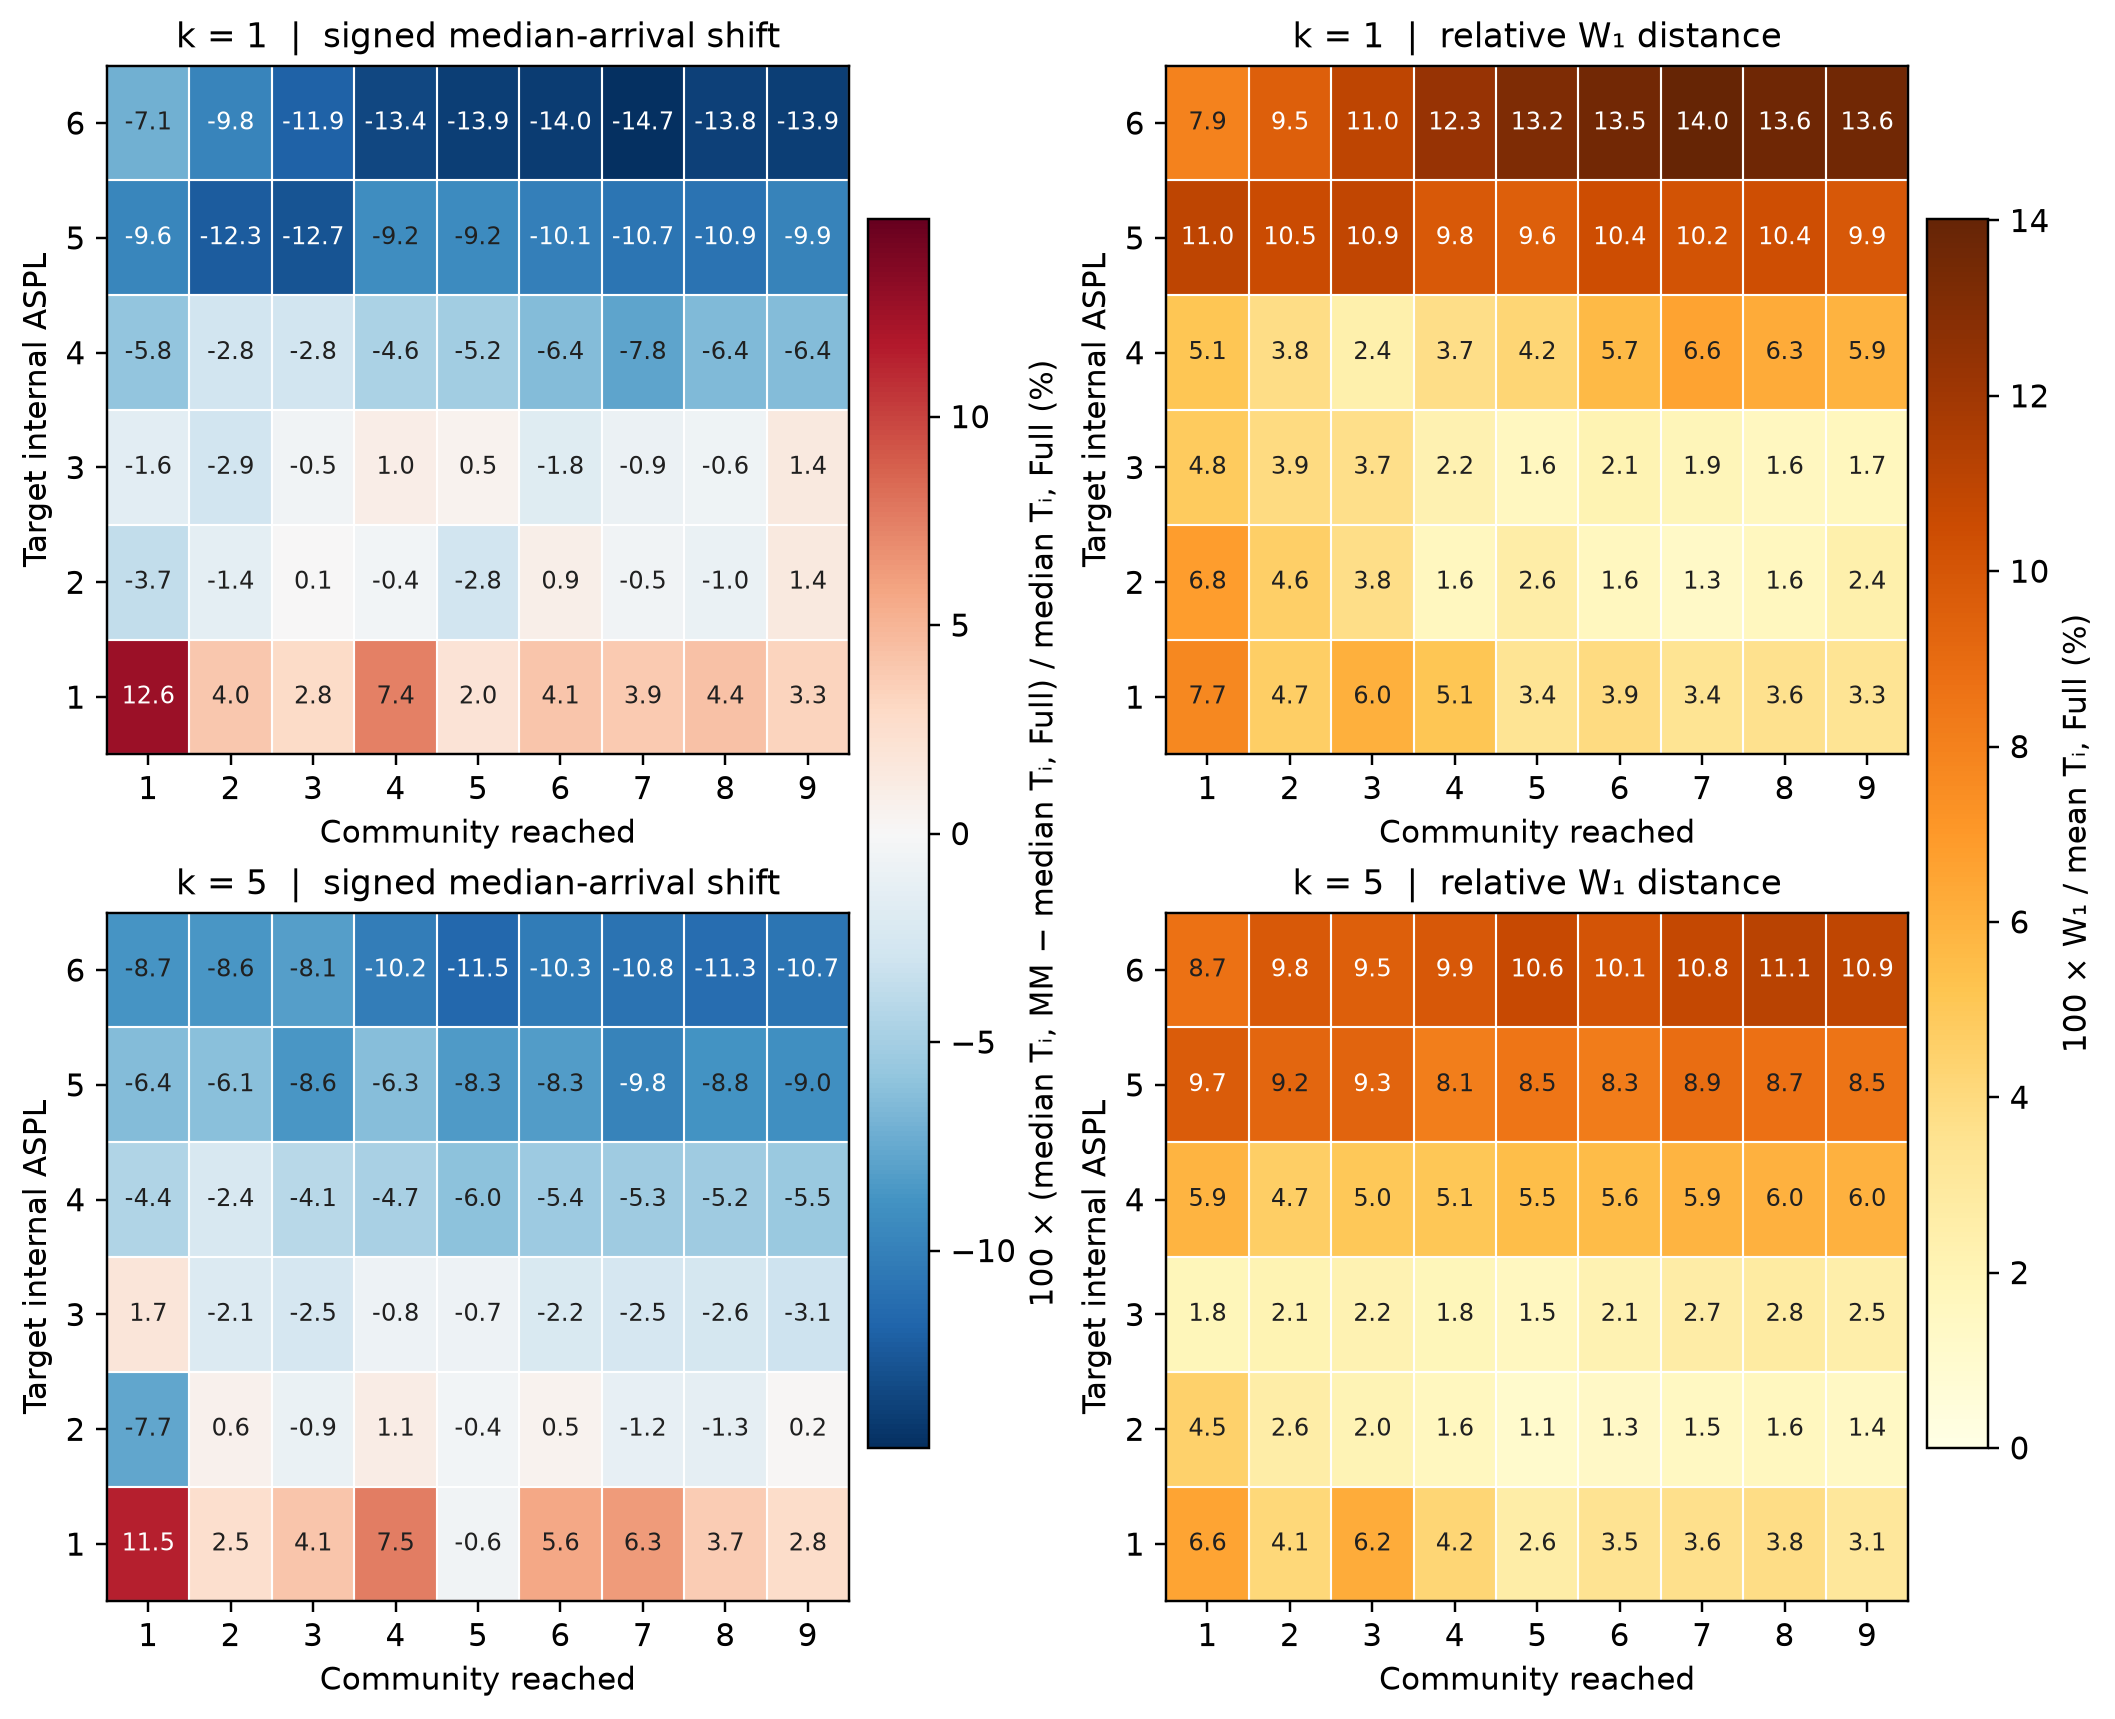
\includegraphics[width=0.82\linewidth]{Images/aspl_chain/aspl_chain_median_arrival_error_map_labeled.png}
\caption{Точність кумулятивних часів прибуття у ланцюгах із десяти спільнот, кожна з яких має $n=1000$ вузлів, залежно від цільового ASPL (рядки) та досягнутої спільноти ($c=1,\dots,9$, стовпці), для $k=1$ (угорі) та $k=5$ (унизу). Ліворуч: відносний зсув медіани $b_c$ (від'ємний: \TS{} прибуває раніше). Праворуч: відносна відстань Васерштайна. Для кожної комірки використано 400 парних запусків; невизначеність не показано (термінальні прибуття див. на рисунку~\ref{fig:accuracy_map}).}
\label{fig:chain_heatmap}
\end{figure}

\subsection{Розмір спільноти та ширина інтерфейсу}
\label{sec:res_size}

\emph{Та сама довжина внутрішнього шляху є значно менш сприятливою в малих спільнотах.} На рисунку~\ref{fig:accuracy_map} наведено термінальну розбіжність для всіх 48 конфігурацій серії за розміром. Пермутаційний поріг був у межах від 1.6\% до 5.9\%. У 16 конфігураціях з ASPL $\le2$ значення $\eW$ становило 1.1--4.4\%, а в 14 із них воно не відрізнялося від порога на рівні значущості 5\%. У 31 із 32 конфігурацій з ASPL $\ge3$ значення $\eW$ перевищувало поріг ($p<0.01$), а зсув медіани був від'ємним із блоковим бутстреп-інтервалом, що не містив нуль. Винятком була конфігурація $n=1000$, ASPL 3, $k=1$, для якої $\eW=1.7\%$. За фіксованого ASPL $\ge3$ розбіжність монотонно зменшувалася зі збільшенням розміру спільноти для обох ширин інтерфейсу. За ASPL 6 значення $\eW$ зменшилося з 41.3\% для $n=50$ до 13.6\% для $n=1000$ за $k=1$, а за $k=5$ --- з 32.4\% до 10.9\%. Ширші інтерфейси зменшували розбіжність у розріджених спільнотах, але не усували її. Частка переходів \TS{}, що передували зараженню будь-якого вузла-моста у спільноті-джерелі, зросла з 0.1--2.3\% за ASPL 1 до 30--52\% за ASPL 6.

\clearpage
\begin{figure}[H]
\centering
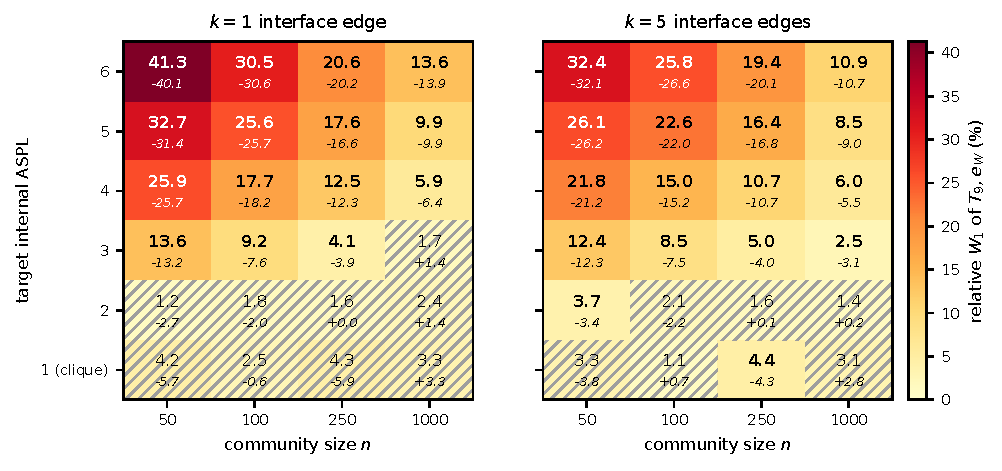
\includegraphics[width=\linewidth]{Images/twoscale/fig_accuracy_map.pdf}
\caption{Точність термінального прибуття у ланцюгах із десяти спільнот для всіх 48 конфігурацій серії за розміром. Колір і напівжирні числа: відносна відстань Васерштайна $\eW$ для $T_9$ (\%). Числа курсивом: відносний зсув медіани $b_9$ (\%; від'ємне значення означає, що \TS{} прибуває раніше). Заштриховані комірки: $\eW$ не відрізняється від внутрішньопарного пермутаційного порога ($p\ge0.05$). Для кожної комірки використано 400 парних запусків.}
\label{fig:accuracy_map}
\end{figure}

\subsection{Єдине співвідношення часових масштабів упорядковує розбіжність}
\label{sec:res_descriptor}

\emph{Якщо виразити результати через $\rho=\beta\sigma_T$, дані для всіх розмірів, структур і ширин інтерфейсу лягають на одну криву.} Для кожної конфігурації ми обчислювали $\sigma_T$ як стандартне відхилення часів зараження вузлів у кожній спільноті-джерелі запусків \Full{}, усереднене за спільнотами й запусками. На рисунку~\ref{fig:descriptor}(a,b) термінальні $\eW$ і $b_9$ зображено залежно від $\rho$. Рангова кореляція між $\eW$ і $\rho$ становила 0.92 для всіх 48 конфігурацій і 0.98 для 32 конфігурацій з ASPL $\ge3$; відповідні значення для цільового ASPL становили 0.82 і 0.67. У 18 конфігураціях із $\rho<0.25$ виконувалося $\eW\le4.4\%$, а 15 із них були нерозрізнюваними з пермутаційним порогом. Усі 30 конфігурацій із $\rho\ge0.25$ були статистично відмінними від порога. Для $\rho\ge0.3$ апроксимація в логарифмічних координатах дала $\eW\approx15\rho\,\%$ (нахил 1.03; медіанне відносне відхилення 8\%, максимальне 41\%) і $b_9\approx-\eW$, тобто розбіжність майже повністю була раннім зсувом. Ми також розглянули два альтернативні масштабування: $\beta\sqrt{k}\sigma_T$, запропоноване виразом~\eqref{eq:hazard_variance}, і середній час від першого зараження спільноти до зараження її першого вузла-моста, помножений на $\beta k$. Обидва розділяли дві ширини інтерфейсу сильніше, ніж $\rho$.

\clearpage
\begin{figure}[H]
\centering
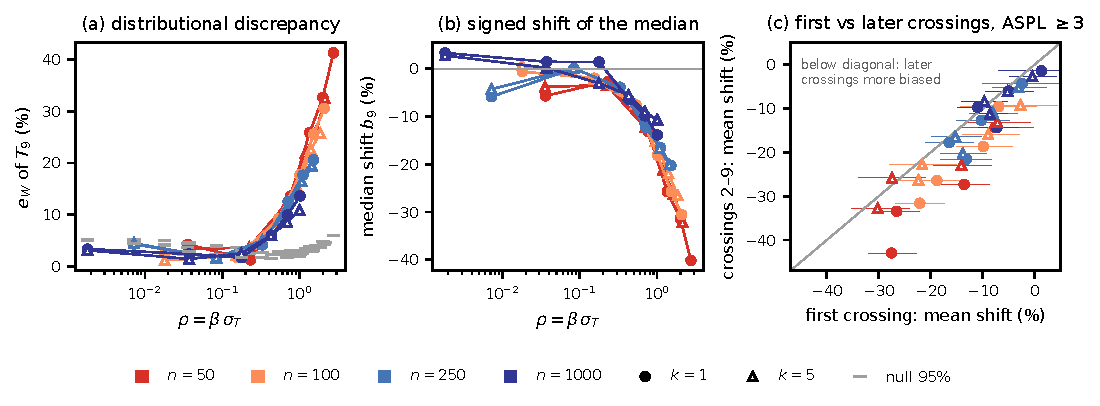
\includegraphics[width=\linewidth]{Images/twoscale/fig_descriptor.pdf}
\caption{(a) Відносна відстань Васерштайна та (b) відносний зсув медіани термінального прибуття залежно від $\rho=\beta\sigma_T$ для всіх 48 конфігурацій ланцюга (кольори: розмір спільноти; зафарбовані кола: $k=1$; порожні трикутники: $k=5$; лінії сполучають ASPL 1--6 за фіксованих $n$ і $k$). Сірі позначки в (a): 95-й процентиль внутрішньопарного пермутаційного порога кожної конфігурації. (c) Локальний середній зсув першого переходу порівняно зі зсувом переходів 2--9 для конфігурацій з ASPL $\ge3$, із 95\% блоковими бутстреп-інтервалами зсуву першого переходу.}
\label{fig:descriptor}
\end{figure}

Рисунок~\ref{fig:descriptor}(c) розділяє окремі переходи. Згідно із зауваженням~\ref{rem:placement}, у нашому дизайні перший перехід залежить лише від механізмів на боці джерела та чисельних механізмів, тоді як наступні переходи також залежать від розміщення після першого імпорту й надлишкових імпортів. Для $k=1$ наступні переходи мали сильніше зміщення, ніж перший, у 15 із 16 конфігурацій з ASPL $\ge3$. Різниця була статистично відмінною від нуля у 9 з них, зокрема для всіх чотирьох розмірів за ASPL 6; наприклад, $-27.5\%$ для першого переходу порівняно з $-42.9\%$ для переходів 2--9 за $n=50$. Для $k=5$ різниця була меншою (14 із 16 точкових оцінок від'ємні, 3 статистично відмінні від нуля). Така залежність від $k$ відповідає передбаченню механізму вичерпання інтерфейсу: одне фізичне ребро допускає один перехід, тоді як п'ять ребер допускають до п'яти, тому надлишкові агреговані імпорти мають менший вплив. Оскільки між конфігураціями використано спільне випадкове засівання, ми вважаємо цю закономірність підтверджувальним, але не остаточним свідченням. Безпосередній підрахунок надлишкових імпортів потребував би журналів типів подій, які не зберігалися.

%======================================================================
\clearpage
\section{Обговорення}
\label{sec:discussion}

\subsection{Практичні рекомендації}

Результати дають змогу запропонувати просту процедуру для визначення того, чи є агреговане зв'язування достатнім.

\paragraph{Визначте, яка спостережувана величина має значення.}
Для часу поширення між спільнотами двомасштабний симулятор може бути точним. Для маршрутів передачі йому довіряти не можна. До половини переходів у розріджених спільнотах і п'ята частина експортів навіть там, де розподіли часу експорту узгоджувалися, відбувалися до зараження будь-якого справжнього вузла-моста. Питання, що залежать від вузлів-мостів, як-от спрямування втручань на осіб, які з'єднують спільноти, або встановлення джерела спалаху, потребують інформації про межу, якої агрегований інтерфейс не містить.

\paragraph{Оцініть співвідношення часових масштабів.}
Обчисліть $\rho=\beta_{\mathrm{out}}\sigma_T$. Оскільки $\sigma_T$ описує поширення в межах однієї спільноти, його в принципі можна оцінити лише за локальними рушіями, моделюючи ізольовану спільноту з рівномірно розміщеним початковим інфікованим вузлом. Ми обчислювали його за еталонними запусками й не перевіряли таку локальну оцінку. У наших тестах термінальні часи прибуття були статистично нерозрізнюваними за $\rho\lesssim0.25$. Для $0.3\lesssim\rho\lesssim3$ модель \TS{} прибувала раніше приблизно на $15\rho\%$. Це правило є емпіричним узагальненням для одного сімейства синтетичних мереж і параметрів, а не загальним законом похибки.

\paragraph{Перевіряйте абсолютні та відносні похибки.}
Уздовж ланцюга відносна розбіжність була майже сталою, тому абсолютне випередження у віддалених спільнотах зростало пропорційно часу поширення. Для визначення часу втручання в конкретній цільовій спільноті релевантною величиною є абсолютна розбіжність у цій спільноті.

\paragraph{Калібруйте відстані відносно вибіркової мінливості.}
За кількох сотень запусків для кожної моделі відстані в кілька відсотків між розподілами часу прибуття очікуються навіть для ідентичних моделей (додаток~\ref{app:floor}). Такі порівняння слід доповнювати пермутаційними базовими рівнями або аналітичними порогами.

\subsection{Обчислювальна вартість}
\label{sec:disc_cost}

Тести було розроблено для оцінювання точності, тому їхні явні інтерфейси містять не більше п'яти ребер, а повна еталонна модель є обчислювально недорогою. У цьому режимі агрегація майже не усуває обчислювальної роботи, а домінує вартість синхронізації на часовій сітці. Медіанний час виконання одного повтору Python-реалізацій був у межах 0.04--0.07\,с (\Full{}) і 0.6--31\,с (\TS{}) для $n=50$ та 8.6--18\,с і 6.7--124\,с відповідно для $n=1000$. Для $n=1000$ відношення двох медіан було в межах від 0.76 (ASPL 2, $k=5$) до 6.9 (ASPL 6, $k=1$). Із цього випливають два висновки. По-перше, коли повна мережа відома й невелика, слід віддавати перевагу \Full{}. По-друге, накладні витрати двомасштабного методу зумовлені планувальником типу «чорна скринька», а не агрегацією. Подієвий планувальник, який точно інтегрує кусково-сталу інтенсивність (розділ~\ref{sec:timing}), усунув би як ці накладні витрати, так і похибку синхронізації. Обчислювальний виграш очікується, коли міжспільнотні контакти численні або недоступні, тобто в умовах, для яких метод і призначено~\citep{kuryliak2025towards}; його кількісне оцінювання залишено для майбутніх досліджень.

\subsection{Обмеження}

В експериментах використано SI-динаміку. За наявності одужання вузли-мости можуть припинити передачу, тоді як частка інфікованих у всій спільноті залишається додатною; у такому разі агрегована інтенсивність також може переоцінювати експорт на пізній стадії локального спалаху. Усі мережі синтетичні, макротопологія є ланцюгом, а внутрішні й зовнішні інтенсивності на ребро однакові. Інтерфейси розміщувалися випадково, що згідно із зауваженням~\ref{rem:placement} нейтралізує похибку розміщення для перших імпортів. Структуровані інтерфейси, наприклад із мостами у вузлах-концентраторах або з віддаленими один від одного вхідними й вихідними мостами, можуть поводитися інакше. Крок синхронізації не варіювали, тому чисельну складову розбіжності не було виокремлено; твердження~\ref{prop:surrogate} дає прямий спосіб зробити це. Нарешті, $\rho$ оцінювали за еталонними запусками й обрали з невеликої кількості можливих масштабувань; його прогностичну цінність для інших сімейств мереж ще потрібно перевірити.

\subsection{Можливі розширення}

Аналіз указує на модифікації, що використовують лише агреговану інформацію. Вичерпання інтерфейсу можна представити, обмеживши кількість імпортів через кожен пучок кількістю його каналів, яка відома, якщо $W_{ij}$ підраховує ребра, або зменшуючи $\lambda_{ij}$ у міру вичерпання цієї місткості. Якщо доступна часткова інформація про межу, $\ibar_i$ у~\eqref{eq:macro_rate} можна замінити часткою інфікованих серед відомих вузлів-мостів. Тоді розміщення можна обмежити відомими кінцевими вузлами-отримувачами. Кожен такий варіант можна порівняти з \Full{} і з точним моделюванням на $\tilde G$, що дає змогу відокремити модельну похибку від чисельної.

%======================================================================
\clearpage
\section{Висновки}
\label{sec:conclusions}

Двомасштабний метод зв'язує точні локальні рушії Gillespie через агреговані інтенсивності між спільнотами. В ідеальній формі він є точним моделюванням на сурогатній мережі, у якій кожен інтерфейс рівномірно розподілено між усіма парами вузлів. Це визначає, яку інформацію метод втрачає: стан справжніх вузлів-мостів, розташування імпортів і скінченну пропускну здатність тонких інтерфейсів. Для випадково розміщених інтерфейсів звідси також випливає, що агреговані годинники експорту стохастично випереджають точні. У контрольованих порівняннях із Gillespie-моделюванням повної мережі розподіли часу термінального прибуття були статистично нерозрізнюваними, коли інфекція поширювалася спільнотами швидко порівняно з часом, потрібним для переходу через ребро інтерфейсу. Коли внутрішній розкид часу наближався до часу такого переходу або перевищував його, двомасштабний симулятор систематично прибував раніше; похибка сягала 40\% у малих розріджених спільнотах. Співвідношення $\rho=\beta\sigma_T$ упорядкувало ці результати для різних розмірів спільнот, внутрішніх структур і ширин інтерфейсу. Близькі часи ніколи не гарантували допустимих маршрутів передачі. Отже, метод є обґрунтованим інструментом для питань про час поширення за малого $\rho$. Він не придатний для питань про індивідуальні маршрути передачі або для розріджених спільнот із довгими внутрішніми шляхами без уточнення інтерфейсу.

%======================================================================
\appendix

\clearpage
\section{Формули для кліки та перевірка}
\label{app:clique}

Розглянемо кліку з $n$ вузлів із SI-динамікою, інтенсивністю $\beta$ на ребро, рівномірно розміщеним початковим інфікованим вузлом і рівномірно вибраною множиною з $k$ вузлів-мостів. Коли заражено $m$ вузлів, наступне внутрішнє зараження відбувається з інтенсивністю $\beta m(n-m)$ незалежно від того, які саме вузли заражені, а множина заражених є рівномірною $m$-підмножиною. Імовірність того, що серед перших $m$ заражених вузлів немає жодного моста, дорівнює $\binom{n-k}{m}/\binom{n}{m}$, отже
\begin{equation}
\label{eq:clique_TB}
\mathbb{E}[T_B]=\sum_{m=1}^{n-k}\frac{\binom{n-k}{m}}{\binom{n}{m}}\frac{1}{\beta m(n-m)},
\qquad
\mathbb{E}[T_B]=\frac{H_{n-1}}{\beta n}\ \ (k=1),
\end{equation}
де $H_{n-1}$ --- гармонічне число; випадок, коли початковий інфікований вузол є мостом ($T_B=0$), також ураховано. Для $k=1$ час експорту у \Full{} дорівнює $T_B$ плюс незалежний час очікування $\Exp(\beta)$. Очікуваний час зараження всієї кліки дорівнює $2H_{n-1}/(\beta n)$. У таблиці~\ref{tab:verification} вираз~\eqref{eq:clique_TB} порівняно з першою спільнотою ланцюгів клік.

\clearpage
\begin{table}[H]
\centering
\caption{Перевірка еталонного симулятора на першій спільноті ланцюгів клік ($\beta=0.003$, 400 запусків для кожної комірки): середній час активації моста та, для $k=1$, середній час очікування після активації (точне значення $1/\beta=333.3$). Наведено середнє $\pm$ стандартна похибка.}
\label{tab:verification}
\small
\begin{tabular}{rrrrr}
\toprule
$n$ & $k$ & $\mathbb{E}[T_B]$, рівн.~\eqref{eq:clique_TB} & середнє $T_B$ у \Full{} & очікування у \Full{} після $T_B$\\
\midrule
50 & 1 & 29.86 & $29.72\pm0.71$ & $354.0\pm16.9$\\
100 & 1 & 17.26 & $17.05\pm0.38$ & $326.5\pm17.0$\\
250 & 1 & 8.13 & $7.84\pm0.15$ & $347.4\pm16.6$\\
1000 & 1 & 2.49 & $2.51\pm0.04$ & $353.8\pm17.9$\\
50 & 5 & 15.97 & $15.96\pm0.55$ & --\\
100 & 5 & 10.31 & $9.64\pm0.29$ & --\\
250 & 5 & 5.35 & $5.16\pm0.12$ & --\\
1000 & 5 & 1.80 & $1.77\pm0.03$ & --\\
\bottomrule
\end{tabular}
\end{table}

\clearpage
\section{Вибірковий поріг відстані Васерштайна}
\label{app:floor}

Нехай $F_R$ і $G_R$ --- емпіричні функції розподілу двох незалежних вибірок розміру $R$ з одного неперервного розподілу $F$. Тоді $W_1=\int|F_R-G_R|\,dx$, а $\sqrt{R}\,(F_R-G_R)$ наближено дорівнює $\sqrt{2}$, помноженому на броунівський міст, обчислений у $F(x)$~\citep{delbarrio1999}. Оскільки $\mathbb{E}|B(u)|=\sqrt{2u(1-u)/\pi}$ для броунівського мосту $B$,
\[
\mathbb{E}[W_1]\approx\frac{2}{\sqrt{\pi R}}\int\sqrt{F(x)\bigl(1-F(x)\bigr)}\,dx .
\]
Для експоненційного розподілу із середнім $\mu$ інтеграл дорівнює $\mu\pi/2$, тому $\mathbb{E}[W_1]/\mu\approx\sqrt{\pi/R}$, що становить 8.9\% для $R=400$ і 1.8\% для $R=10\,000$. Часи прибуття, що є сумами кількох переходів, мають менший розкид відносно свого середнього, а тому й нижчий поріг; пермутаційні пороги конфігурацій ланцюга були в межах від 1.6\% до 5.9\%.

\clearpage
\section{Відомості про відтворюваність}
\label{app:repro}

Значення seed детерміновано отримано з параметрів експерименту. Кожен рушій \TS{} використовує власний потік псевдовипадкових чисел; зондування в середині кроку копіюють стан потоку свого рушія й не просувають його. Два запуски \Full{} ($n=50$, ASPL 6, $k=1$) не досягли десятої спільноти до $T=30\,000$. Їх було повторно запущено до $T=40\,000$ з тими самими графами, початковими вузлами та seed подій. Було перевірено, що їхні історії подій до 30\,000 збігаються зі збереженими запусками, а термінальні прибуття відбулися приблизно в моменти 31\,059 і 31\,007. Значення горизонту не підставляли замість неспостереженої події. Пермутаційний і бутстреп-аналіз конфігурацій ланцюга, дескриптор $\sigma_T$ і рисунки~\ref{fig:accuracy_map}--\ref{fig:descriptor} було обчислено зі збережених запусків скриптами \path{extrascripts/analysis/smpt_twoscale_paper_metrics.py} і \path{extrascripts/visualization/smpt_twoscale_paper_figures.py}.

%======================================================================
\section*{Заява про внесок авторів за CRediT}
\textbf{Yulian Kuryliak:} Концептуалізація, методологія, програмне забезпечення, дослідження, формальний аналіз, візуалізація, написання --- початкова версія. \textbf{Michael T. M. Emmerich:} Концептуалізація, методологія, наукове керівництво, написання --- рецензування та редагування. [Автори мають підтвердити.]

\section*{Декларація про конфлікт інтересів}
Автори заявляють, що їм не відомо про будь-які конкуруючі фінансові інтереси або особисті відносини, які могли б вплинути на роботу, описану в цій статті.

\section*{Фінансування}
[Інформацію про фінансування мають додати автори.]

\section*{Доступність даних}
Код симуляції, збережені результати симуляцій і скрипти аналізу доступні у відповідального автора за обґрунтованим запитом. [Замінити на DOI репозиторію, якщо дані буде депоновано.]

\section*{Декларація про використання генеративного штучного інтелекту та технологій на основі ШІ під час підготовки рукопису}
Під час підготовки цієї роботи автори використовували [назва інструмента або сервісу] з метою [причина]. Після використання цього інструмента або сервісу автори перевірили й за потреби відредагували вміст та беруть на себе повну відповідальність за зміст опублікованої статті. [Автори мають заповнити.]

